%%%%%%%%%%%%%%%%%%%%%%%%%%%%%%%%%%%%%%%%%%%%%%%%%%%%%%%%%%%%%%%%%%%%%%%%
\chapter{Trace-Driven Simulator}
%%%%%%%%%%%%%%%%%%%%%%%%%%%%%%%%%%%%%%%%%%%%%%%%%%%%%%%%%%%%%%%%%%%%%%%%


To generate traces for the simulation, \SIM uses Pin~\cite{pin} for
x86 traces and GPUOcelot~\cite{ocelot} for PTX traces. Both traces are
converted to internal RISC style micro-ops (uop) and those uops are
simulated. Figure~\ref{fig:overview} shows the overview of \SIM
simulator.


\begin{figure*}[htb]
\centering 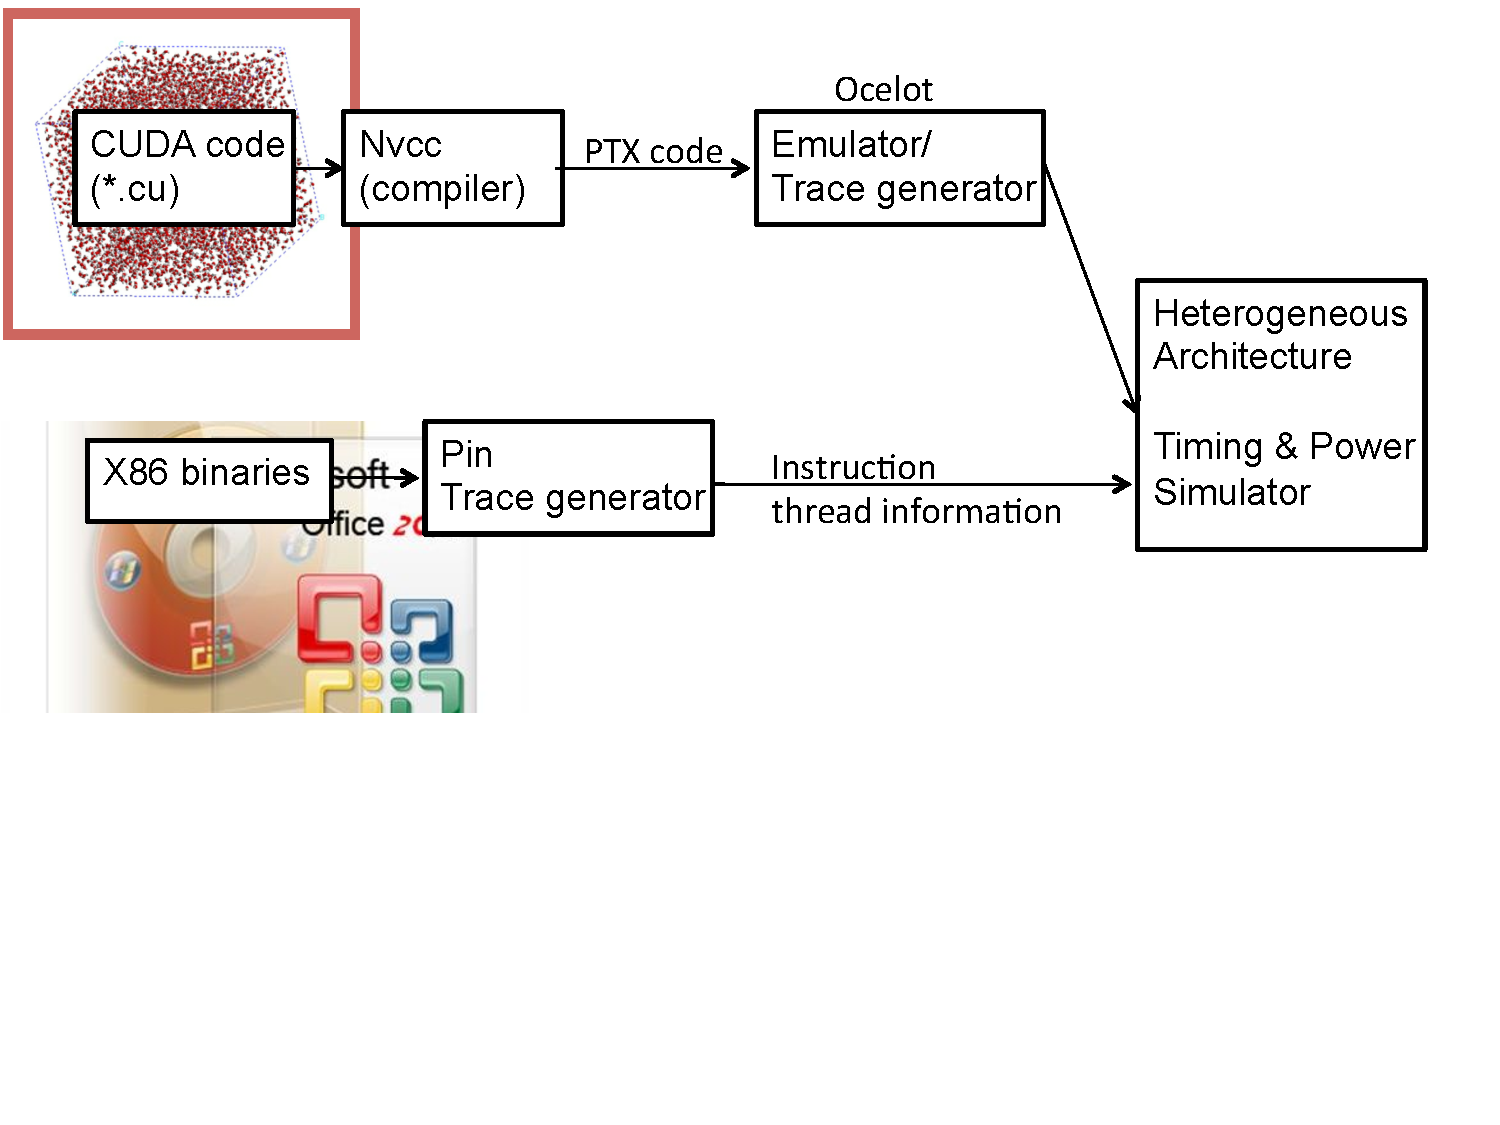
\includegraphics{figs/macsim_overview}
\caption{The overview of MacSim Simulator}
\label{fig:overview}
\end{figure*}


%%%%%%%%%%%%%%%%%%%%%%%%%%%%%%%%%%%%%%%%%%%%%%%%%%%%%%%%%%%%%%%%%%%%%%%%
%\section{Trace Generation}
%\label{sec:trace_generation}
%%%%%%%%%%%%%%%%%%%%%%%%%%%%%%%%%%%%%%%%%%%%%%%%%%%%%%%%%%%%%%%%%%%%%%%%



%%%%%%%%%%%%%%%%%%%%%%%%%%%%%%%%%%%%%%%%%%%%%%%%%%%%%%%%%%%%%%%%%%%%%%%%
\section{CPU (X86) Traces}
%%%%%%%%%%%%%%%%%%%%%%%%%%%%%%%%%%%%%%%%%%%%%%%%%%%%%%%%%%%%%%%%%%%%%%%%

CPU (X86) traces are generated with the aid of Pin~\cite{pin}, a
binary instrumentation tool.  The detail descriptions of Pin including
installation can be found in \urlc{http://www.pintool.org}.  We provide
\cpu trace generator within \SIM repository. After installing
Pin\footnote{Note that our CPU trace generator may not be
  backward/forward compatible with the pin version. Currently, pin
  41150 revision (Jun 07, 2011) must be used.}, we need to build the
X86 trace generator module (trace\_generator.so), which can be simply
done with the following commands.



\begin{Verbatim}
cd toos/x86_trace_generator
make
\end{Verbatim}

\noindent
The above will create trace\_generator.so in the
tools/x86\_trace\_generator/obj-intel64 directory.  Then, MacSim X86
traces can be generated by running pin along with the module.


\begin{Verbatim}
pin -t trace_generator.so -- $BIN $ARGS (for single-threaded)
pin -t trace_generator.so -thread N -- $BIN $ARGS (for multi-threaded)
\end{Verbatim}


The following shows the example of the trace generation for /bin/ls. 
With the command of 

\begin{Verbatim}
pin -t trace\_generator.so -- /bin/ls
\end{Verbatim}

\noindent
, the binary (ls) is actually executed on top of the pin and the
instructions executed at run-time are stored into the trace
file. Following is the example outputs when we generate a `ls' command
trace:


\begin{Verbatim}
pin -t trace_generator.so -- /bin/ls
-> Thread[0->0] begins.
-> Trace Generation Starts at icount 0
dump.txt_0.dump  pin.log  trace_0.raw  trace_generator.o  trace_generator.so  
xed_extractor.o  xed_extractor.so
-> Trace Generation Done at icount 475195
\end{Verbatim}


After the trace generation is done, Trace.txt and trace\_0.raw are
created in the directory. Section~\ref{sec:traceformat} details
generated trace files.



%%%%%%%%%%%%%%%%%%%%%%%%%%%%%%%%%%%%%%%%%%%%%%%%%%%%%%%%%%%%%%%%%%%%%%%%
\section{GPU (PTX) Traces}
\label{sec:gpu_traces}
%%%%%%%%%%%%%%%%%%%%%%%%%%%%%%%%%%%%%%%%%%%%%%%%%%%%%%%%%%%%%%%%%%%%%%%%

GPU (PTX) traces are generated using Ocelot~\cite{ocelot}, which is a dynamic compilation
framework for heterogeneous system. 


%%%%%%%%%%%%%%%%%%%%%%%%%%%%%%%%%%%%%%%%%%%%%%%%%%%%%%%%%%%%%%%%%%%%%%%%
\subsection{Installing Ocelot}
%%%%%%%%%%%%%%%%%%%%%%%%%%%%%%%%%%%%%%%%%%%%%%%%%%%%%%%%%%%%%%%%%%%%%%%%

Ocelot can be installed either using ubuntu packages provided by the official
page or via its SVN repository. To install the latest version, check out 
source files using the following command:


\begin{Verbatim}
svn checkout http://gpuocelot.googlecode.com/svn/trunk/ gpuocelot
\end{Verbatim}


After checking out source files, you can build Ocelot and trace generator libraries using the following commands:


\begin{Verbatim}
cd gpuocelot/ocelot; sudo ./build.py --install
cd gpuocelot/trace-generators; libtoolize; aclocal; autoconf; automake; ./configure; 
make; sudo make install
\end{Verbatim}


%%%%%%%%%%%%%%%%%%%%%%%%%%%%%%%%%%%%%%%%%%%%%%%%%%%%%%%%%%%%%%%%%%%%%%%%
\subsection{Generating Traces}
%%%%%%%%%%%%%%%%%%%%%%%%%%%%%%%%%%%%%%%%%%%%%%%%%%%%%%%%%%%%%%%%%%%%%%%%

CUDA executables which are targeted to generate traces should be linked against
libocelot.so and libocelotTrace.so.

In order to generate traces, the following four environment variables need to be set.

\begin{itemize}\itemsep2pt
\item TRACE\_PATH : directory to store generated traces. If not specified, current directory is used by default.
\item TRACE\_NAME : prefix name for generated traces. If not specified, "Trace" is used by default.
\item KERNEL\_INFO\_PATH : file that contains kernel information (must be specified)
\item COMPUTE\_VERSION : compute capability (must be specified)
\end{itemize}

The following shows an example of how to set up the environment variables.


\begin{Verbatim}
export TRACE_PATH="/storage/traces/"  # Create a trace directory in the /storage/traces
export KERNEL_INFO_PATH="kernel_info" # kernel_info has the kernel information
export COMPUTE_VERSION="2.0"          # Calculate occupancy based on compute capability 2.0
\end{Verbatim}


The kernel information file (kernel\_info) should contain the following
information: kernel name, register usage (per thread), and shared memory usage
(per thread).


\begin{Verbatim}
_Z9Memcpy_SWPfS_i 14 52 
\end{Verbatim}


Running CUDA application creates a directory with the kernel name, where traces 
are generated, and kernel\_config.txt which is a configuration used for MacSim.


\begin{Verbatim}
drwxr-xr-x   2 anonymous group 69632 Sep 00 22:03 _Z9Memcpy_SWPfS_i_0
-rw-r--r--   1 anonymous group    66 Sep 09 22:29 kernel_config.txt
\end{Verbatim}



%%%%%%%%%%%%%%%%%%%%%%%%%%%%%%%%%%%%%%%%%%%%%%%%%%%%%%%%%%%%%%%%%%%%%%%%
\section{Supporting Other Architecture}
%%%%%%%%%%%%%%%%%%%%%%%%%%%%%%%%%%%%%%%%%%%%%%%%%%%%%%%%%%%%%%%%%%%%%%%%

To support other architectures, for example AMD processors or ARM
processors, we need a frontend simulator or functional emulator. Using
instruction streams provided by the frontend, we also need to traslate
each instruction to \SIM-internal RISC style micro-ops. Currently, we
plan to provide ARM-based architectures.


%%%%%%%%%%%%%%%%%%%%%%%%%%%%%%%%%%%%%%%%%%%%%%%%%%%%%%%%%%%%%%%%%%%%%%%%
\section{Trace Format}
\label{sec:traceformat}
%%%%%%%%%%%%%%%%%%%%%%%%%%%%%%%%%%%%%%%%%%%%%%%%%%%%%%%%%%%%%%%%%%%%%%%%

There are mainly two different kinds of files in both X86 and PTX traces as
below, which will be explained in the following subsections.

\begin{itemize}\itemsep2pt
\item Trace.txt (info trace): contains the outline information of the trace (\#thread, trace type, ...).
\item Trace\_xx.raw (raw trace): contains instructions for a thread and is generated for each thread (warp\footnote{A warp consists of 32 threads in CUDA.} in case of GPU)
\end{itemize}



%%%%%%%%%%%%%%%%%%%%%%%%%%%%%%%%%%%%%%%%%%%%%%%%%%%%%%%%%%%%%%%%%%%%%%%%
\subsection{Trace.txt}
%%%%%%%%%%%%%%%%%%%%%%%%%%%%%%%%%%%%%%%%%%%%%%%%%%%%%%%%%%%%%%%%%%%%%%%%


\begin{figure*}[htb]
\centering
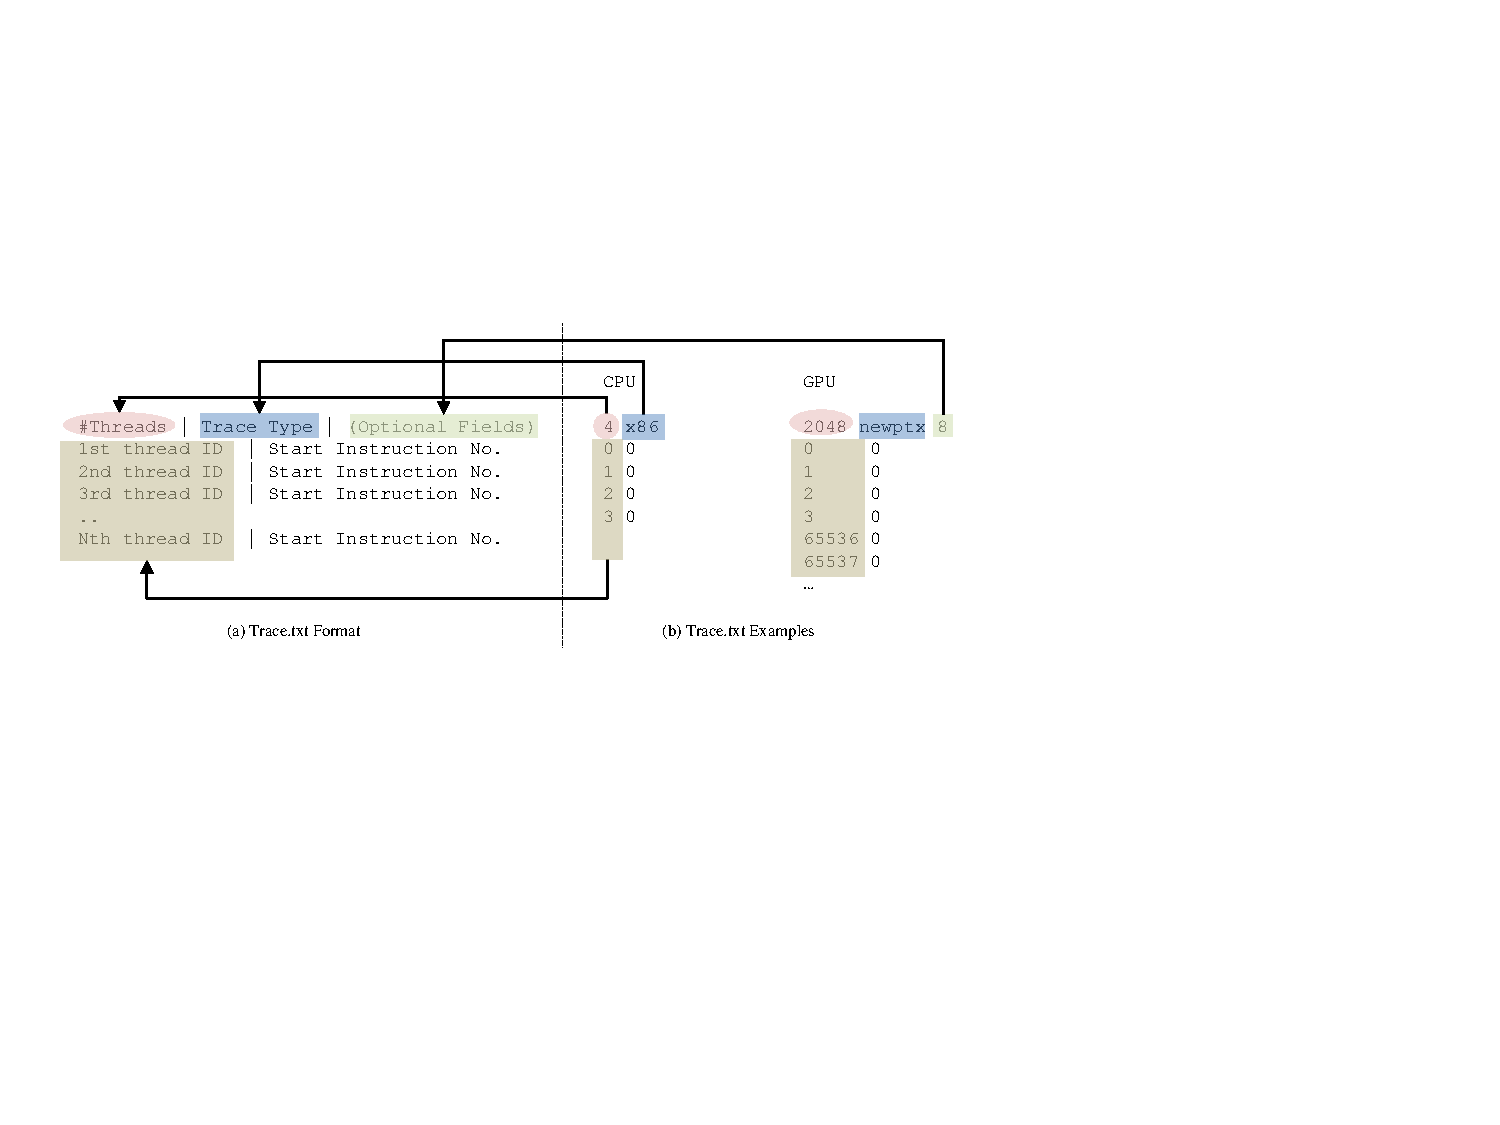
\includegraphics{figs/trace_format}
\caption{Trace.txt format.}
\label{fig:trace_format}
\end{figure*}

Figure~\ref{fig:trace_format} shows the format of Trace.txt and its CPU and GPU
examples.  As shown in Figure~\ref{fig:trace_format}-(a), the first line in the
Trace.txt file has different fields from the rest of lines.

\begin{itemize}\itemsep2pt
\item \#Threads: indicates the number of threads whose trace is generated, and the value 
is the same as the number of following lines. 
\item Trace Type: indicates whether the generated trace is either x86 or ptx.
\item Optional Fields: are currently used for PTX traces, which indicates the number of thread blocks
which will be assigned to a streaming multiprocessor(SM) core (occupancy).
\end{itemize}

From the second line, there are two fields in each line: thread ID and start
instruction number.  For each thread ID, there exists a trace\_xx.raw where
dynamic instructions for the thread are stored. Finally, Start Instruction No.
indicates the number of instructions to skip when executing instructions in the
Trace\_xx.raw file.

For instance, in Figure~\ref{fig:trace_format}-(b), we can see that the CPU
trace has four threads and its type is set to x86. Optional Fields are not used 
since they are only for GPU traces. We also know that Trace\_0.raw$-$Trace\_3.raw 
exist because \#Thread indicates that there are raw traces for four threads. 
Finally, for each raw trace, we start to execute instructions from the beginning
since the Start Instruction No. field is zero.

In the GPU example, the number of raw traces are 2048 since \#Threads is 2048.
Note that \#Threads indeed means \#Warp in case of GPU traces, so that raw traces
are generated for each warp. In addition, the optional field implies that eight 
thread blocks can be assigned to a SM core. 

In the GPU trace, thread ID is calculated by thread block ID * 65536 + warp ID (in a block). 
In the example, warps 0, 1, 2 and 3 are comprised of a thread block, and warps 65536, 65537, 65538
and 65539 forms another thread block.

%%%%%%%%%%%%%%%%%%%%%%%%%%%%%%%%%%%%%%%%%%%%%%%%%%%%%%%%%%%%%%%%%%%%%%%%
\subsection{Trace\_xx.raw}
%%%%%%%%%%%%%%%%%%%%%%%%%%%%%%%%%%%%%%%%%%%%%%%%%%%%%%%%%%%%%%%%%%%%%%%%

Trace\_xx.raw is generated for each thread/warp and contains a raw information
of dynamic instructions executed for the thread. This raw trace contains various
information such as opcode and source registers for each instruction, whose format 
is the same between x86 and PTX traces and looks as follows:


\begin{Verbatim}
trace format for an instruction in trace_xx.raw

nSR | nDR | SR_IDs | DR_IDs | BrType | bImm | Opcode | bStore | bFP | WF | nLD | InstSize |
LAddr_1 | LAddr_2 | SAddr | PCAddr | BrAddr | MemRSize | MemWSize | RepDir | BrActT 
\end{Verbatim}


Table~\ref{table:trace_desc} summarizes the size of each field and its description.
Note that the raw trace is compressed with zlib to reduce the size when generated, and
the size of each field in the table is before the compression.

\begin{table*}[htb]
\begin{footnotesize}
\begin{center}
\caption{Descriptions of each field in the trace.}
\label{table:trace_desc}
\begin{tabular}{|l|l|l|} 
\hline
Field     & Size (Bytes)       & Description \\ \hline \hline
nSR       & 1                  & number of source registers \\ \hline
nDR       & 1                  & number of destination registers \\ \hline
SR\_IDs   & 9                  & source register IDs \\ \hline
DR\_IDs   & 6                  & destination register IDs \\ \hline
BrType    & 1                  & branch type \\ \hline
bImm      & 1                  & indicates whether this instruction has immediate field \\ \hline
Opcode    & 1                  & opcode \\ \hline
bStore    & 1                  & indicates whether this instruction has store operation \\ \hline
bFP       & 1                  & indicates whether this instruction is FP operation \\ \hline
WriteFlag & 1                  & write flag \\ \hline
nLD       & 1                  & number of load operations \\ \hline
InstSize  & 1                  & instruction size \\ \hline
LAddr\_1  & 4                  & load address 1 \\ \hline
LAddr\_2  & 4                  & load address 2 \\ \hline
SAddr     & 4                  & store address \\ \hline
PCAddr    & 4                  & PC address \\ \hline
BrAddr    & 4                  & branch target address \\ \hline
MemRSize  & 4                  & memory read size \\ \hline
MemWSize  & 1                  & memory write size \\ \hline
RepDir    & 1                  & repetition direction  \\ \hline
BrActT    & 1                  & indicates whether branch is actually taken \\ \hline

\end{tabular}
\end{center}
\end{footnotesize}
\end{table*}

%%%%%%%%%%%%%%%%%%%%%%%%%%%%%%%%%%%%%%%%%%%%%%%%%%%%%%%%%%%%%%%%%%%%%%%%
\subsection{kernel\_config.txt (only for PTX)}
%%%%%%%%%%%%%%%%%%%%%%%%%%%%%%%%%%%%%%%%%%%%%%%%%%%%%%%%%%%%%%%%%%%%%%%%

For PTX traces, as described in Section~\ref{sec:gpu_traces}, a directory is
created for each kernel invocation, where Trace.txt and Trace\_xx.raw are
generated. Since typical GPU applications usually invoke several kernels (or
    execute the same kernel repeatedly), PTX traces can have multiple kernel
directories. Thus, in order to simulate all invoked kernels for a GPU
application, the PTX trace generator creates kernel\_config.txt which contains
the information of invoked kernels.


\begin{Verbatim}
/trace/ptx/parboil/bfs
drwxr-xr-x  4  4096 Sep 21 13:21 .
drwxr-xr-x 11  4096 Sep 13 18:02 ..
drwxr-xr-x  2  4096 Apr  7  2011 _Z17BFS_in_GPU_kernelPiS_P4int2S1_S_S_iS_ii_0
drwxr-xr-x  2  4096 Apr  7  2011 _Z26BFS_kernel_multi_blk_inGPUPiS_P4int2S1_S_S_S_S_iiS_S_S__0
-rw-r--r--  1   184 Apr  7  2011 kernel_config.txt

In kernel_config.txt

-1 newptx
/trace/ptx/parboil/bfs/_Z17BFS_in_GPU_kernelPiS_P4int2S1_S_S_iS_ii_0/Trace.txt
/trace/ptx/parboil/bfs/_Z26BFS_kernel_multi_blk_inGPUPiS_P4int2S1_S_S_S_S_iiS_S_S__0/Trace.txt
\end{Verbatim}


As shown above, all the invoked kernels are enumerated in kernel\_config.txt.
The first line indicates that this is a wrapper file which contains (multiple) trace.txt files, and
the traces are read one by one when finishing the previous trace in MacSim.
In the above example (bfs), kernel\_config.txt indicates that there are two different
kernels in bfs, each of which was invoked once. When running a GPU simulation, we put 
the kernel\_config.txt file into trace\_file\_list (Section~\ref{sec:trace_file_list}). 
Also, we can simulate specific kernels by modifying the kernel\_config.txt file.

%%%%%%%%%%%%%%%%%%%%%%%%%%%%%%%%%%%%%%%%%%%%%%%%%%%%%%%%%%%%%%%%%%%%%%%%
\subsection{Trace for micro-ops}
%%%%%%%%%%%%%%%%%%%%%%%%%%%%%%%%%%%%%%%%%%%%%%%%%%%%%%%%%%%%%%%%%%%%%%%%

While running a simulation, each instruction in the \emph{raw trace} is converted 
into one or more micro-ops internally. MacSim stores such decoded micro-uops into a MacSim-specific
trace structure to facilitate the simulation by populating each field, which is shown 
in Table~\ref{table:trace_uops}.

\begin{table*}[htb]
\begin{footnotesize}
\begin{center}
\caption{MacSim-specific data structure for micro-ops.}
\label{table:trace_uops}
\begin{tabular}{|l|l|l|} 
\hline
Type      & Variable                 & Description \\ \hline \hline
uint8\_t  & m\_opcode                & opcode \\ \hline
Uop\_Type & m\_op\_type              & type of operation \\ \hline
Mem\_Type & m\_mem\_type             & type of memory instruction \\ \hline
Cf\_Type  & m\_cf\_type              & type of control flow instruction \\ \hline
Bar\_Type & m\_bar\_type             & type of barrier caused by instruction \\ \hline
uns       &   m\_num\_dest\_regs     & number of destination registers written \\ \hline
uns       &   m\_num\_src\_regs      & number of source registers read \\ \hline
uns       &   m\_mem\_size           & number of bytes read/written by a memory instruction \\ \hline
uns       &   m\_inst\_size          & instruction size \\ \hline
Addr      &   m\_addr                & pc address  \\ \hline
reg\_info\_s&   m\_srcs[MAX\_SRCS]   & source register information \\ \hline
reg\_info\_s&   m\_dests[MAX\_DESTS] & destination register information \\ \hline
Addr      &   m\_va;                 & virtual address \\ \hline
bool      &   m\_actual\_taken       & branch actually taken \\ \hline
Addr      &   m\_target              & branch target address \\ \hline
Addr      &   m\_npc                 & next pc address  \\ \hline
bool      &   m\_pin\_2nd\_mem       & has second memory operation \\ \hline
inst\_info\_s& *m\_info              & pointer to the instruction hash table  \\ \hline
int       &   m\_rep\_uop\_num       & repeated uop number \\ \hline
bool      &   m\_eom                 & end of macro \\ \hline
bool      &   m\_alu\_uop            & alu uop  \\ \hline
uint32\_t  &   m\_active\_mask       & active mask \\ \hline
uint32\_t  &   m\_taken\_mask        & branch taken mask \\ \hline
Addr      &   m\_reconverge\_addr    & address of reconvergence \\ \hline
bool      &   m\_mul\_mem\_uops      & multiple memory transactions \\ \hline

\end{tabular}
\end{center}
\end{footnotesize}
\end{table*}

\ignore{
The following shows the data structure for micro-uops. 


\begin{Verbatim}
  uint8_t      m_opcode;        /**< opcode */
  Uop_Type     m_op_type;       /**< type of operation */
  Mem_Type     m_mem_type;      /**< type of memory instruction */
  Cf_Type      m_cf_type;       /**< type of control flow instruction */ 
  Bar_Type     m_bar_type;      /**< type of barrier caused by instruction */
  uns          m_num_dest_regs; /**< number of destination registers written */
  uns          m_num_src_regs;  /**< number of source registers read */
  uns          m_mem_size;      /**< number of bytes read/written by a memory instruction */
  uns          m_inst_size;     /**< instruction size */
  Addr         m_addr;          /**< pc address */ 
  reg_info_s   m_srcs[MAX_SRCS]; /**< source register information */
  reg_info_s   m_dests[MAX_DESTS]; /**< destination register information */
  Addr         m_va;            /**< virtual address */
  bool         m_actual_taken;  /**< branch actually taken */
  Addr         m_target;        /**< branch target address */
  Addr         m_npc;           /**< next pc address */ 
  bool         m_pin_2nd_mem;   /**< has second memory operation */
  inst_info_s *m_info;          /**< pointer to the instruction hash table */ 
  int          m_rep_uop_num;   /**< repeated uop number */
  bool         m_eom;           /**< end of macro */
  bool         m_alu_uop;       /**< alu uop */ 
  // GPU simulation
  uint32_t     m_active_mask;   /**< active mask */
  uint32_t     m_taken_mask;    /**< branch taken mask */
  Addr         m_reconverge_addr; /**< address of reconvergence */
  bool         m_mul_mem_uops;  /**< multiple memory transactions */
\end{Verbatim}

}

% LocalWords:  GPU PTX gpuocelot

%%%%%%%%%%%%%%%%%%%%%%%%%%%%%%%%%%%%%%%%%%%%%%%%%%%%%%%%%%%%%%%%%%%%%%%%%%%%%%%%%%%%%%

\ignore{
\begin{table*}[htb]
\begin{footnotesize}
\begin{center}
\caption{MacSim trace format.}
\label{table:trace_format}
\begin{tabular}{|l|l|} 
\hline
Type               & Description \\ \hline 
uint8\_t           & number of source registers \\ \hline
uint8\_t           & number of destination registers \\ \hline
uint8\_t[9]        & source register IDs \\ \hline
uint8\_t[6]        & destination register IDs \\ \hline
uint8\_t           & branch type \\ \hline
bool               & indicates whether this instruction has immediate field \\ \hline
uint8\_t           & opcode \\ \hline
bool               & indicates whether this instruction has store operation \\ \hline
bool               & indicates whether this instruction is FP operation \\ \hline
bool               & write flag \\ \hline
uint8\_t           & number of load operations \\ \hline
uint8\_t           & instruction size \\ \hline
uint32\_t          & load address 1 \\ \hline
uint32\_t          & load address 2 \\ \hline
uint32\_t          & store address \\ \hline
uint32\_t          & PC address \\ \hline
uint32\_t          & branch target address \\ \hline
uint32\_t          & memory read size \\ \hline
uint8\_t           & memory write size \\ \hline
uint8\_t           & repetition direction  \\ \hline
uint8\_t           & indicates whether branch is actually taken \\ \hline

\end{tabular}
\end{center}
\end{footnotesize}
\end{table*}
}

\ignore{
\begin{table*}[htb]
\begin{footnotesize}
\begin{center}
\caption{MacSim trace format.}
\label{table:trace_format}
\begin{tabular}{|l|l|l|l|l|l|l|l|l|l|l|l|l|l|l|l|} 
\hline
nSR & nDR & SR\_IDs & DR\_IDs & BrType & bImm & Opcode & bStore & bFP & WF & nLD  \\ \hline \hline
InstSize & LAddr\_1 & LAddr\_2 & SAddr & PCAddr & BrAddr & MemRSize & MemWSize & RepDir & BrActT & \\ \hline
\end{tabular}
\end{center}
\end{footnotesize}
\end{table*}

Tables~\ref{table:trace_format} and ~\ref{table:trace_desc} show the trace
format for each instruction and the description of each field, respectively.
}



